\section{Expected Value \& Variance}
Let $X$ be a continuous (potentially very complicated) random variable with PDF $f$. Suppose we were asked to pick \emph{one real number} $\mu$, subject to a certain constraint, that best represents the random variable $X$. Of course, note that $X$ is a random variable and might be very different than just one single (deterministic) real number. That being said, we want to try our best to pick said real number that satisfies this constraint.

\subsection{Expected Value}
One natural thing to do is to pick a $\mu$ so that best represents the random variable (i.e., is closest to the random variable). So, we can consider the \emph{squared distance}. In particular, we want to find a $\mu$ such that \[(X - \mu)^2\] is likely to be as close to 0 as possible. Note that $(X - \mu)^2$ is itself a random variable. Put it another way, we want to find a $\mu$ that minimize the random distance $(X - \mu)^2$. So, we want to minimize 
\[\int_{-\infty}^{\infty} (x - \mu)^2 f(x) dx.\]
By linearity, we have 
\begin{equation*}
    \begin{aligned}
        \int_{-\infty}^{\infty} (x - \mu)^2 f(x) dx &= \int_{-\infty}^{\infty} (x^2 - 2x\mu + \mu^2) f(x) dx \\ 
            &= \int_{-\infty}^{\infty} x^2 f(x) dx - 2\mu \int_{-\infty}^{\infty} xf(x) dx + \mu^2 \int_{-\infty}^{\infty} f(x) dx. 
    \end{aligned}
\end{equation*} 
Since $f(x)$ is a PDF, the third integral is just 1. Hence, we want to minimize 
\[\int_{-\infty}^{\infty} x^2 f(x) dx - 2\mu \int_{-\infty}^{\infty} xf(x) dx + \mu^2.\]
Differentiating with respect to $\mu$, we get 
\[-2 \int_{\infty}^{\infty} xf(x) dx + 2\mu.\]
If we set this equal to 0 and then solve for $\mu$, we find the minimizer is 
\[\mu = \int_{-\infty}^{\infty} xf(x) dx.\]
We note that $\mu$ is a \textbf{weighted average}. We integrate over all possible values of $x$, and then weigh them by their corresponding density $f(x)$. 

\begin{definition}{Expected Value}{}
    Suppose that $X$ is a continuous random variable with PDF $f$. Then, the \textbf{expected value} (or \textbf{mean}) of $X$ is 
    \[\mu = \mathbb{E}(X) = \int_{-\infty}^{\infty} xf(x)dx.\]
\end{definition}
\textbf{Remarks:} 
\begin{itemize}
    \item For some random variables, this expected value (integral) does not exist. We won't need to worry about this here, though. 
    \item If $X$ is a \textbf{discrete} random variable with PMF $p(x) = \PR(X = x)$, then $\mu = \mathbb{E}(X) = \sum_{x} xp(x)$. 
\end{itemize}
The \textbf{mean} $\mu$ gives us valuable information about the ``center'' of a distribution. This, along with \textbf{standard deviation} $\mu$ (which tells us about the ``spread'' of a distribution), tells us the fundamental quantities in regards to the ``shape'' of a distribution. 

\begin{mdframed}[]
    (Example.) Suppose we roll a fair die, which takes values between 1 and 6, each with equal probability $\frac{1}{6}$. Then, 
    \[\mu = \sum_{k = 1}^{6} k \cdot \frac{1}{6} = \frac{1}{6} \sum_{k = 1}^{6} k = \frac{7}{2}.\]
    Here, we're considering all possible values that the die can take (from $k = 1$ to 6). Each value has a probability of $\frac{1}{6}$. 

    \bigskip 

    While $\frac{7}{2}$ is not a value that the random variable can actually take (note that the random variable can only take values 1, 2, 3, 4, 5, and 6), but in some sense it is the expected value, or the average value. To see why this is the case, consider the following histogram:  
    \begin{center}
        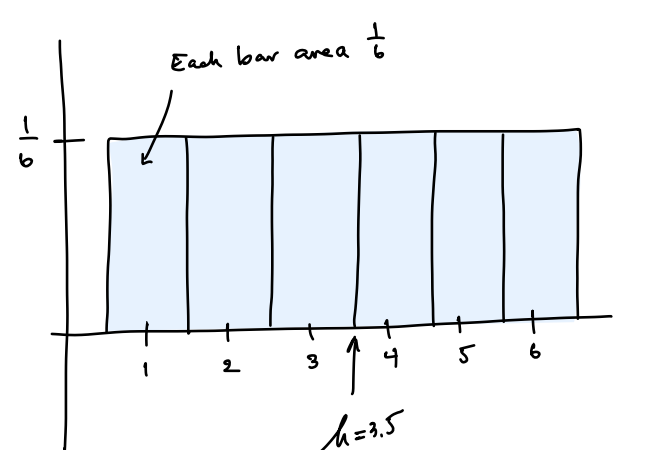
\includegraphics[scale=0.7]{assets/lec14die.png}
    \end{center} 
    We can think of the 3.5 mark as the ``center of mass.''
\end{mdframed}

\begin{theorem}{Law of Unconscious Statistics (LotUS)}{}
    Suppose that $X$ is a random variable and $\phi: \R \mapsto \R$ is a function. Then, 
    \begin{enumerate}
        \item If $X$ is continuous with PDF $f$, then 
        \[\mathbb{E}[\phi(X)] = \int_{-\infty}^{\infty} \phi(x) f(x) dx.\]

        \item If $X$ is discrete with PMF $p$, then 
        \[\mathbb{E}[\phi(X)] = \sum_{x} \phi(x) p(x).\]
    \end{enumerate}
\end{theorem}
\textbf{Remarks:} 
\begin{itemize}
    \item It is enough \emph{just} to know the PDF/PMF of $X$ to find the expected value of $Y = \phi(X)$.
    \item This shows us that expectation is linear. In particular, the \textbf{Linearity of Expectation} (LoE) says that if we let $X$ be a random variable, then we can suppose that $a, b \in \R$. Then, $\mathbb{E}(aX + b) = a\mathbb{E}(X) + b$. 
\end{itemize}
\textbf{Warning:}
\begin{itemize}
    \item LoE does not imply that $\mathbb{E}(XY) = \mathbb{E}(X) \mathbb{E}(Y)$. 
    \item Note that this is true if $X$ and $Y$ are independent, but not true otherwise. 
\end{itemize}

\subsection{Variance}
\begin{definition}{Variance}{}
    The \textbf{variance} of a random variable $X$, denoted by $\sigma^2 = \text{Var}(X)$, is the expected squared distance of $X$ from its mean $\mu$. That is, $\sigma^2 = \mathbb{E}[(X - \mu)^2]$. 
\end{definition}
\textbf{Remarks:}
\begin{itemize}
    \item This is telling us about the \emph{spread} of the distribution; that is, how far away should we expect the random variable to be away from its mean. 
    \item Recall that the mean $\mu$ is the real number that minimizes $\mathbb{E}[(X - a)^2]$ over all real numbers $a$. Whatever this quantity happens to be at the minimizer $a = \mu$ is called the variance $\sigma^2$. 
\end{itemize}

\begin{theorem}{}{}
    Let $X$ be a random variable and let $a, b \in \R$. Then, 
    \[\text{Var}(aX + b) = a^2\text{Var}(X) = a^2 \mathbb{E}[(X - \mu)^2].\]
\end{theorem}
\textbf{Remark:} Note that the variance of a constant is 0, since the distribution of a constant random variable has no ``spread'' at all. 

\textbf{Warning:} While expected value is linear, variance is not. In other words, if $X$ and $Y$ are \emph{independent}, then $\text{Var}(X + Y) = \text{Var}(X) + \text{Var}(\text{Y})$. However, this is not true in general. 

\bigskip 

Note that the formula $\sigma^2 = \mathbb{E}[(X - \mu)^2]$ is useful conceptually, but not so convenient for computations. Instead, we can use the Linearity of Expectation to obtain the following, more convenient, formula: 
\[\sigma^2 = \mathbb{E}(X^2 - 2\mu X + \mu^2) = \mathbb{E}(X^2) - 2\mu \mu + \mu^2 = \mathbb{E}(X^2) - \mu^2.\]
Therefore, the \textbf{computational variance formula} is given by 
\[\boxed{\text{Var}(X) = \mathbb{E}(X^2) - [\mathbb{E}(X)]^2}.\]
The quantity $\mathbb{E}(X^2)$ is called the \textbf{second moment} of $X$, and can be computed using LotUS. That is, if $X$ is continuous, then 
\[\mathbb{E}(X^2) = \int_{-\infty}^{\infty} x^2 f(x) dx.\]
If $X$ is discrete, then 
\[\mathbb{E}(X^2) = \sum_{x} x^2 p(x).\]

\subsection{Standard Deviation}
\begin{definition}{Standard Deviation}{}
    The square root of the variance, $\sigma = \sqrt{\text{Var}(X)}$, is called the \textbf{standard deviation} of $X$.
\end{definition}
The reason for the name is that, for ``most reasonable'' distributions, the ``bulk'' of the mass/density deviates by at most $\sigma$ from the center $\mu$. That is, usually, ``most'' of the mass/density is on the values of 
\[x \in [\mu - \sigma, \mu + \sigma].\]

\begin{theorem}{Chebyshev's Inequality}{}
    Let $X$ be a random variable with \emph{both} mean $\mu$ and standard deviation $\sigma$. Then, for any real number $a > 0$, we have that 
    \[\PR(|X - \mu| \geq a \sigma) \leq \frac{1}{a^2}.\]
\end{theorem}
\textbf{Remarks:}
\begin{itemize}
    \item In other words, for any distribution with a mean and variance, the probability that $X$ is at least $a = 2$ standard deviations from the center $\mu$ of the distribution is at most $\frac{1}{4}$.
    \item For many distributions, the actual probability is \emph{much} smaller. However, this is an useful upper bound that works for all distributions.
\end{itemize}
This result follows by 
\begin{theorem}{Markov's Inequality}{}
    Let $X$ be a non-negative random variable, i.e. $\PR(X \geq 0) = 1$, with mean $\mu$ and $b > 0$ a positive number. Then, $\PR(X \geq b) \leq \frac{\mu}{b}$. 
\end{theorem}

\begin{mdframed}[]
    \begin{proof}
        (Continuous Case.) Since $X$ is non-negative, we know that 
        \[\mu = \int_{-\infty}^{\infty} xf(x) dx = \int_0^{\infty} xf(x) dx.\]
        Splitting the integral, we have 
        \[\int_{0}^{b} xf(x) dx + \int_{b}^{\infty} xf(x) dx \geq \int_{b}^{\infty} xf(x) dx \geq b \int_{b}^{\infty} f(x) dx = b \PR(X \geq b).\]
        Hence, $\PR(X \geq b) \leq \frac{\mu}{b}$, as claimed.
    \end{proof}
\end{mdframed}

\subsection{Examples of Finding Expected Value and Variance}

\begin{mdframed}[]
    (Example.) If $X$ is Bernoulli($p$), then $\mu = p$ and $\sigma^2 = pq$, where $q = 1 - p$. Then, 
    \[\mathbb{E}(X) = 1 \cdot p + 0 \cdot q = p.\]
    Note that $X^2$ has the same distribution as $X$, since $X$ only takes the values $0 = 0^2$ and $1 = 1^2$. Hence, $\mathbb{E}(X^2) = \mathbb{E}(X) = p$. Hence, 
    \[\text{Var}(X) = p - p^2 = p(1 - p) = pq.\]
\end{mdframed}

\begin{mdframed}[]
    (Example.) If $X$ is Binomial($n, p$), then it is the sum of $n$ independent Bernoulli($p$) trials. By the Linearity of Expectation, we know that 
    \[\mathbb{E}(X) = np.\]
    Since the trials are \emph{independent}, we have that 
    \[\text{Var}(X) = npq.\]
\end{mdframed}
Note that this is the special case of the following fact. 
\begin{theorem}{}{}
    Suppose that $X_1, \dots, X_n$ are IID with mean $\mu$ and variance $\sigma^2$. Then, their sum $S_n = \sum_{k = 1}^{n} X_k$ has mean $\mathbb{E}(S_n) = n\mu$ and variance $\text{Var}(S_n) = n\sigma^2$. 
\end{theorem}

\begin{mdframed}[]
    (Example.) If $X$ is Geometric($p$), then $\mathbb{E}(X) = \frac{1}{p}$. So, if $p$ is really small, then we should expect to wait a while before our first success; likewise, if $p$ is large, then we may not need to wait long before our first success. This is intuitive; in particular, the probability of success is $p$, so we should expect about 1 success in every $p$ trials. But, intuition aside, there are several ways to compute this.
    \begin{itemize}
        \item Approach 1.
        \begin{mdframed}[]
            \[\mathbb{E}(X) = \sum_{k = 1}^{\infty} kpq^{k - 1} = p\sum_{k = 1}^{\infty} kq^{k - 1}.\]
            Recall that this is a \emph{geometric} random variable, so we will use the geometric series; in particular, 
            \[\sum_{k = 0}^{\infty} q^k = \frac{1}{1 - q}\]
            and 
            \[\sum_{k = 1}^{\infty} kq^{k - 1} = \frac{d}{dq} \sum_{k = 0}^{\infty} q^k.\]
            Hence,
            \[\mathbb{E}(X) = p \frac{d}{dq} \frac{1}{1 - q} = p\frac{1}{(1 - q)^2} = \frac{p}{p^2} = \frac{1}{p}.\] 
            Similarly, we can show that $\text{Var}(X) = \frac{q}{p^2}$. 
        \end{mdframed}

        \item Approach 2. 
        \begin{mdframed}[]
            Let $X$ be the number of trials until the first success. Then, we have 
            \[\mathbb{E}(X) = 1p + (1 + \mathbb{E}(X))q.\]
            Solving for $\mathbb{E}(X)$ gives us the desired solution.
        \end{mdframed}
    \end{itemize}
\end{mdframed}

\begin{mdframed}[]
    (Example.) A Poisson($\lambda$) has mean and variance $\mu = \sigma^2 = \lambda$. So, 
    \[\mathbb{E}(X) = \sum_{k = 0}^{\infty} ke^{-\lambda} \frac{\lambda^k}{k!} = \sum_{k = 1}^{\infty} e^{-\infty} \frac{\lambda^k}{(k - 1)!} = \lambda \sum_{k = 0}^{\infty} e^{-\lambda} \underbrace{\frac{\lambda^k}{k!}}_{1} = \lambda.\]
    Similarly, you can show that $\mathbb{E}(X^2) = \lambda(1 + \lambda)$ so that $\text{Var}(X) = \lambda(1 + \lambda) - \lambda^2 = \lambda$. 
\end{mdframed}

\begin{mdframed}[]
    (Example.) An Exponential($\lambda$) has $\mu = \frac{1}{\lambda}$ and $\sigma^2 = \frac{1}{\lambda^2}$. For this computation, the theorem following this example will be useful. 

    \bigskip 
    
    If $X$ is Exponential($\lambda$), then it is non-negative and $\PR(X > x) = e^{-\lambda x}.$ Hence, 
    \[\mathbb{E}(X) = \int_{0}^{\infty} e^{-\lambda x} dx = \frac{1}{\lambda}.\]
\end{mdframed}

\begin{theorem}{Expectation Tail Sum for Non-Negative Random Variables}{}
    If $X$ is a non-negative random variable (i.e., $\PR(X \geq 0) = 1$), then 
    \begin{enumerate}
        \item If $X$ is discrete, then 
        \[\mathbb{E}(X) = \sum_{k = 0}^{\infty} \PR(X > k).\]

        \item If $X$ is continuous, then 
        \[\mathbb{E}(X) = \int_{0}^{\infty} \PR(X > x) dx.\]
    \end{enumerate}
\end{theorem}

\begin{mdframed}[]
    \begin{proof}
        (Discrete.) Just note that 
        \begin{equation*}
            \begin{aligned}
                \mathbb{E}(X) &= \sum_{k = 0}^{\infty} kp(k) \\ 
                    &= p(1) + (p(2) + p(2)) + (p(3) + p(3) + p(3)) + \dots \\ 
                    &= (p(1) + p(2) + p(3) + \dots) + (p(2) + p(3) + \dots) + (p(3) + \dots) + \dots \\
                    &= \PR(X > 0) + \PR(X > 1) + \PR(X > 2) + \dots
            \end{aligned}
        \end{equation*}
        Hence, we're done.
    \end{proof}
\end{mdframed}

\begin{mdframed}[]
    (Example.) If $X$ is Normal($\mu, \sigma^2$), then, indeed, $\mu$ is the mean and $\sigma^2$ is its variance. To see why this is the case, see lecture slides.
\end{mdframed}

\begin{mdframed}[]
    (Example.) If $X$ is Cauchy, then $\mathbb{E}(X)$ does not exist. Recall that a (standard) Cauchy has PDF 
    \[f(x) = \frac{1}{\pi(1 + x^2)}.\]
    Note that 
    \[\int_{-\infty}^{\infty} \frac{x}{\pi (1 + x^2)}dx\]
    diverges, since
    \[\int_{0}^{\infty} \frac{x}{1 + x^2}dx = \infty.\]
\end{mdframed}

\subsection{Conditional Expectation}
Recall that if $X$ is a discrete random variable with PMF $p$, and $B$ is an event with $\PR(B) > 0$, then 
\[p(x | B) = \frac{p(x)}{\PR(B)}\]
is a probability distribution on $B$. This is the PMF of the random variable $X$, given $B$. 

\begin{definition}{}{}
    Let $X$ be a random variable with PMF $p$. Suppose that $\PR(B) > 0$. Then, the conditional expectation of $X$ given $B$ is 
    \[\mathbb{E}(X | B) = \sum_{x} xp(x | B).\]    
\end{definition}
\textbf{Remark:} The situation is similar in the continuous case, but we instead have a conditional PDF 
\[f(x | B) = \frac{f(x)}{\PR(B)}\]
and the conditional expectation is given by  
\[\mathbb{E}(X | B) = \int_{-\infty}^{\infty} xp(x | B) dx.\]  


\subsubsection{Law of Total Expectation}
Just like how there is a Law of Total Probability, there is also a Law of Total Expectation. 
\begin{theorem}{Law of Total Expectation}{}
    Let $X$ be a random variable on sample space $\Omega$. Suppose that $B_1, \dots, B_n$ is a partition $\Omega$. Then, 
    \[\mathbb{E}(X) = \sum_{i = 1}^{n} \mathbb{E}(X | B_i) \PR(B_i).\]
\end{theorem}
This is useful because, often, $\mathbb{E}(X)$ is sometimes difficult to find directly. However, if we condition on a well-chosen $B_i$, then it becomes manageable. 

\begin{mdframed}[]
    (Example.) In the gambling game ``craps,'' a player makes a bet and then rolls a pair of dice. If the sum is 7 or 11, the player wins. If it is 2, 3, or 12, the player loses. If the sum is any other number $s$, the player continues to roll until either another $s$ (they win) or 7 (they lose) occurs (7 is lucky the first time). Now, let $R$ be the number of rolls in a single game of craps.
    \begin{enumerate}
        \item Find $\mathbb{E}(R)$. 
    \end{enumerate}

    \begin{mdframed}[]
        \begin{enumerate}
            \item By the Law of Total Expectation, we have 
            \[\mathbb{E}(R) = \sum_{x = 2}^{12} \mathbb{E}(R | X = x)\PR(X = x),\]
            where $X$ is the initial sum. Note that if 
            \[x \in \{2, 3, 7, 11, 12\},\]
            then \[\mathbb{E}(R | X = x) = 1\]
            since the game is immediately over if we get one of those numbers. In particular,
            \begin{itemize}
                \item There is 1 way to get a 2 (11).
                \item There are 2 ways to get a 3 (12, 21).
                \item There are 6 ways to get a 7 (16, 61, 25, 52, 43, 34).
                \item There are 2 ways to get a 11 (56, 65).
                \item There is 1 way to get a 12 (66).
            \end{itemize}
            Hence, 
            \[\sum_{x \in \{2, 3, 7, 11, 12\}} \mathbb{E}(R | X = x) \PR(X = x) = \frac{12}{36}.\]
            Now, if \[x \in \{4, 5, 6, 8, 9, 10\},\] then we can use a similar argument to the one above. For example, when $x = 4$, we have 3 ways to get 4 (13, 31, 22). This gives us \[\PR(X = 4) = \frac{3}{36}.\] There are also 6 ways to get 7 (16, 61, 25, 52, 43, 34). Therefore, the number of rolls $R$, given that the initial sum is $X = 4$, is distributed as $1 + G$, where $G$ is a geometric random variable (where the success is defined by rolling a 4 or 7) with success probability $p = \frac{9}{36}$. Note that the 1 is there because of the initial roll of the 4, but then we have to keep rolling. Thus, we get  
            \[\mathbb{E}(R | X = 4)\PR(X = 4) = \left(1 + \frac{36}{9}\right) \frac{3}{36}.\]
            To see how we got $\left(1 + \frac{36}{9}\right)$, recall that $E(X) = \frac{1}{p}$ if $X$ is Geometric($p$). So, by Linearity of Expectation, we get that the expected value of 1 (so it's 1) plus the expected value of the geometric (so it's $36 / 9$).

            \bigskip 

            So, by similar reasoning, we get 
            \begin{equation*}
                \begin{aligned}
                    \mathbb{E}(R) = \frac{12}{36} &+ \left(1 + \frac{36}{9}\right) \frac{3}{36} + \left(1 + \frac{36}{10}\right) \frac{4}{36} + \left(1 + \frac{36}{11}\right) \frac{5}{36} \\ 
                        &+ \left(1 + \frac{36}{11}\right) \frac{5}{36} + \left(1 + \frac{36}{10}\right) \frac{4}{36} + \left(1 + \frac{36}{9}\right)\frac{3}{36} = \frac{557}{165} \approx 3.375
                \end{aligned}
            \end{equation*}
            So, on average, we expect a little bit more than 3 and $1/3$ rolls of the dice in each of te game of craps. 
        \end{enumerate}
    \end{mdframed}
\end{mdframed}

\begin{mdframed}[]
    (Example Problem.) Vito is lost in a maze. At the center of the maze, there are 3 paths. Path 1 leads out of the maze after a 2 minute walk. Paths 2 and 3 lead back to the center of the maze after 2 and 3 minute walks, respectively. Suppose that each time Vito is at the center of the maze he picks path $i$ with probability $i/6$. Show that, on average, Vito finds his way out in 15 minutes.

    \bigskip 

    \noindent
    \emph{Hint:} Use ``First Step Analysis.'' That is, use the Law of Total Expectation, with respect to his first choice.

    \begin{mdframed}[]
        First, note that the probability that Vito picks path $i$, $P_i$, is given by 
        \[\PR(P_1) = \frac{1}{6}, \quad \PR(P_2) = \frac{2}{6} = \frac{1}{3}, \quad \PR(P_3) = \frac{3}{6} = \frac{1}{2}.\]
        Let $T$ be the time that Vito gets out of the maze. Then, we have 
        \[\E(T) = \E(T | P_1) \PR(P_1) + \E(T | P_2) \PR(P_2) + \E(T | P_3) \PR(P_3).\]
        Now, we note that 
        \begin{itemize}
            \item $\E(T | P_1) = 2$ is the expected time by taking path 1.
            \item $\E(T | P_2) = 2 + \E(T)$ is the expected time by taking path 2. Note that we add $\E(T)$ because we end up back at the center. 
            \item $\E(T | P_3) = 3 + \E(T)$ is the expected path by taking path 3. Again, note that we add $\E(T)$ because we end up back at the center. 
        \end{itemize}
        Thus, we get 
        \begin{equation*}
            \begin{aligned}
                \E(T) &= 2 \frac{1}{6} + (2 + \E(T)) \frac{1}{3} + (3 + \E(T)) \frac{1}{2} \\ 
                    &\implies \E(T) = \frac{1}{3} + \frac{2}{3} + \frac{1}{3} \E(T) + \frac{3}{2} + \frac{1}{2} \E(T) \\ 
                    &\implies \E(T) - \frac{1}{3} \E(T) - \frac{1}{2} \E(T) = \frac{1}{3} + \frac{2}{3} + \frac{3}{2} \\ 
                    &\implies \E(T) \left(1 - \frac{1}{3} - \frac{1}{2}\right) = \frac{1}{3} + \frac{2}{3} + \frac{3}{2} \\ 
                    &\implies \E(T) = \frac{\frac{1}{3} + \frac{2}{3} + \frac{3}{2}}{1 - \frac{1}{3} - \frac{1}{2}} \\ 
                    &\implies \E(T) = 15,
            \end{aligned}
        \end{equation*}
        as expected.
    \end{mdframed}
\end{mdframed}


\subsubsection{Martingales}
Informally, we can think of martingales as random processes that encapsulate the idea of a \emph{fair game}.
\begin{definition}{}{}
    Let $(X_0, X_1, X_2, \dots)$ be a sequence of random variables and $\phi$ a function. Let $M_n = \phi(X_n)$. The sequence $(M_0, M_1, M_2, \dots)$ is called a \textbf{martingale} (MG) with respect to $(X_0, X_1, X_2, \dots)$ if, for any $n$ and any $x_0, x_1, \dots, x_n$, we have that 
    \[\mathbb{E}(M_{n + 1} - M_{n} | X_{n} = x_n, \dots, X_0 = x_0) = 0.\]
\end{definition}
\textbf{Remark:} If we think of $M_n$ as the total winnings after $n$ bets by a gambler, then $(M_0, M_1, M_2, \dots)$ is a ``fair game'' in the sense that neither the gambler nor the ``house'' has an advantage. In other words, after the $(n + 1)$th game, we would expect no additional gain (hence why this is equal to 0).

\begin{theorem}{}{}
    For any random variables $X$ and $Y$, we have that 
    \[\mathbb{E}[\mathbb{E}(X | Y)] = \mathbb{E}(X).\]
\end{theorem}
\textbf{Remarks:} 
\begin{itemize}
    \item Recall that $\mathbb{E}(M_{n + 1} | X_n, \dots, X_0) = M_n$ for a MG. Then, taking expectations on both sides, it follows that $\mathbb{E}(M_{n + 1}) = \mathbb{E}(M_n)$ for all $n$. Hence, for all (deterministic) times $n \geq 0$, we have that $\mathbb{E}(M_n) = \mathbb{E}(M_0)$. 
    \item These are a powerful tool, which can lead to quick or slick proofs of things that would be computationally challenging otherwise. 
\end{itemize}

\begin{mdframed}[]
    (Example.) Recall, from Lecture 1, that Peter and Paul keeps flipping a coin. If it is ``Heads,'' then Peter wins \$1. Otherwise, Peter loses \$1. Let $X_i$ be Peter's winning after the $i$th bet. Note that $X_0 = 0$.

    \bigskip 

    To see that this is a MG, note that the series of flips are independent. Hence, for any $n$ and any $x_1, \dots, x_n$, we have 
    \[\mathbb{E}(X_{n + 1} - X_{n} | X_n = x_n, \dots, X_1 = x_1) = (1)\frac{1}{2} + (-1) \frac{1}{2} = 0.\]
\end{mdframed}
Recall that $\mathbb{E}(M_n) = \mathbb{E}(M_0)$ for all (deterministic) times $n \geq 0$. However, this is not necessarily true for \emph{random} $T$. Hence, we restrict to a special class of random times. 

\begin{definition}{}{}
    A time $T$ is a \textbf{stopping time} (ST) if and only if, for any $n$, to know if $T = n$, we only need to know the values of $X_0, X_1, \dots, X_n$. That is, we do not need any information about the future after time $n$. 
\end{definition}
For example, the first time we visit 0 is a ST, but the last time we visit 0 is not (in order for us to know if time $n$ is 0, we need to know the full history).

\begin{theorem}{The Optional Stopping Theorem (OST)}{}
    If $(M_0, M_1, \dots)$ is a MG and $T$ is a ST, then $\mathbb{E}(M_T) = \mathbb{E}(M_0)$ if the following conditions are satisfied: 
    \begin{enumerate}
        \item $M_n$ is bounded until time $T$, and 
        \item $\PR(T < \infty) = 1$. 
    \end{enumerate}
\end{theorem}

\begin{mdframed}[]
    (Example: Gambler's Ruin). Suppose that Peter currently has \$1. Furthermore, suppose that they play instead with a coin that comes up Heads with probability $p \neq 1/2$. What is the probability $\PR(J)$ that Peter wins the ``Jackpot'' ($\$N$) before going ``bust'' (\$0)?

    \begin{mdframed}[]
        For this biased RW, we know that \[M_n = (q / p)^{X_n}\] is a MG, where $X_n$ is Peter's winnings. Note that here \[\phi(x) = (q / p)^x.\] Then, 
        \begin{equation*}
            \begin{aligned}
                \mathbb{E}(M_{n + 1} - M_{n} | X_n = x_n, \dots, X_1 = x_1) &= (q / p)^{x_n} (q / p - 1)p + (q / p)^{x_n} (p / q - 1)q \\ 
                    &= (q / p)^{x_n}[(q - p) + (p - q)] \\ 
                    &= 0.
            \end{aligned}
        \end{equation*}
        Now, let $T$ be the first time that $X_n \in \{0, N\}$. By the OST, we know that \[q / p = \mathbb{E}(M_T) = 1 \cdot \PR(J^C) + (q / p)^N \cdot \PR(J).\]
        Hence, \[\PR(J) = \frac{(q / p) - q}{(q / p)^N - 1}.\]
    \end{mdframed}
\end{mdframed}